\section{Software}

\subsection{\textit{Product Design}}

O \textit{design} do produto é o processo que os \textit{designers} usam para combinar as necessidades do usuário com os objetivos de negócio para criar produtos e experiências de sucesso. 

\subsubsection{\textit{User Centered Design}}
\textit{User Centered Design} (Design centrado no usuário) é um termo usado para descrever os processos de \textit{design} os quais os usuários finais influenciam. Alguns processos utilizam técnicas voltadas para entendimento das necessidades dos usuários em pontos específicos, como levantamento de requisitos e testes de usabilidade. Outros métodos têm o usuário como um parceiro dos \textit{designers}, tendo um grande impacto no processo de \textit{design} \cite{abras2004user}.
Para o contexto da disciplina, foram utilizadas algumas técnicas do \textit{User Centered Design} citadas nos tópicos a seguir.

\subsubsubsection{Entrevistas}
Para criar um produto que satisfaça as necessidades dos seus usuários, é necessário entender suas dores e anseios. A realização de entrevistas com usuários é um dos métodos do \textit{User Centered Design} que pode ser utilizado para esse fim.
Existem quatro técnicas bastante difundidas no processo de criação de um produto: entrevistas estruturadas, semi-estruturadas, não estruturadas e por telefone. \cite{wilson2013interview}

\begin{itemize}
\item \textbf{Estruturadas} : Entrevistas com perguntas estruturadas e padronizadas, utilizadas principalmente para reunir dados demográficos, compreender o conhecimento do usuário, ou para reunir dados de atitude e de opinião.
\item \textbf{Semi-estruturadas} : O método de entrevistas semi-estruturadas utiliza uma combinação de perguntas estruturadas com a liberdade exploratória das entrevistas não estruturadas.
Ela é útil quando você tem algum conhecimento sobre um tópico, mas deseja dar aos usuários a oportunidade de levantar novas questões ou quando o tópico é muito complexo para ser uma entrevista estruturada.
\item \textbf{Não estruturadas} : Nas entrevistas não estruturadas, utilizam-se de tópicos gerais; porém, não é necessária nenhuma pergunta ou formato pré determinado. Essa entrevista é extremamente importante pra reunir dados sobre as experiências dos participantes, sem restrições. É uma conversa com um objetivo, e o rumo da entrevista pode ser ditado por ambos os participantes.
\item \textbf{Por telefone} : As entrevistas por telefone são geralmente entrevistas semiestruturadas ou estruturadas conduzidas de maneira remota.
\end{itemize}

Com embasamento nessas técnicas, fizemos algumas entrevistas com nossos \textit{stakeholders}. Aplicamos diferentes técnicas para cada uma das entrevistas, pois os objetivos eram diferentes.
\begin{itemize}
\item \textbf{Entrevista semi-estruturada} : A utilização da entrevista semi estruturada foi feita em um cenário complexo, onde tínhamos pouco conhecimento do assunto.
Foram criadas perguntas simples para dar objetivo inicial para a entrevista. Após isso, os próprios \textit{stakeholders} tocaram a entrevista, e os integrantes do grupo apenas complementavam com perguntas sobre o assunto. 
Essa entrevista serviu para entendermos quais dados eram gerados na simulação e quais valores eles traziam para os \textit{stakeholders}. A partir dessa entrevista, conseguimos entender quais os usos dos dados que seriam coletados e mostrados pelo nosso sistema
\item \textbf{Entrevista não estruturada} : A entrevista não estruturada foi utilizada em um contexto onde já tínhamos um conhecimento melhor sobre o assunto e queríamos validar a experiencia dos usuários com o protótipo criado.
Não foi estruturada nenhuma pergunta ou método, apenas o objetivo: validar o protótipo.
O resultado da entrevista foi uma série de apontamentos sobre a necessidade de cada usuário em cada fase de uma missão. Esses resultados foram utilizados posteriormente para criar uma evolução do protótipo.
\end{itemize}


\subsubsubsection{\textit{Brainwriting}}
Umas das técnicas mais populares para documentar ideias de maneira rápida é o \textit{brainstorm}. No entanto, essa técnica exige muito esforço para ser aplicada em grupo, devido à dificuldade de organização das ideias e ao gerenciamento de conflitos.
O \textit{brainwriting} é a aplicação da técnica do \textit{brainstorm} de maneira silenciosa, proposto para substituir o \textit{brainstorm} em grupos. 
“Brainwriting é a geração silenciosa e escrita de ideias por um grupo de pessoas”. \cite{vangundy1984brain}

Existem 6 maneiras distintas de se fazer um \textit{brainwriting}, são elas:

\begin{itemize}
\item \textit{Nominal Group Technique} (NGT)
\item \textit{Collective Notebook} (CNB)
\item \textit{Brainwriting Pool}
\item \textit{Pin Cards}
\item \textit{Battelle-Bildmappen-Brainwriting} (BBB)
\item \textit{SIL Method}
\end{itemize}

Para execução do \textit{brainwriting} no nosso contexto, foram feitas algumas adaptações a partir do entendimento e da aplicação de cada uma das técnicas.
Foi utilizada uma combinação das técnicas \textit{Brainwriting Pool} e  \textit{Nominal Group Technique} (NGT), resultando na seguinte definição:

\begin{itemize}
\item o organizador deve identificar um tema central da sessão, um problema;
\item cada participante vai usar seu espaço no MIRO para fazer um \textit{brainstorm} silencioso durante 5 minutos cronometrados;
\item após os primeiros 5 minutos, os participantes vão usar o espaço do colega do lado pra fazer suas próprias anotações por mais 5 minutos (pode-se repetir);
\item após a segunda ou terceira interação (dependendo do organizador), cada participante volta para seu espaço e lê suas ideias para o grupo. Nessa etapa, os integrantes podem fazer perguntas e comentários para ajudar a entender melhor a ideia em questão;
\item após todos os integrantes terem lido e entendido o que foi feito, todas as ideias serão agrupadas de acordo com sua similaridade ou proximidade;
\item cada participante receberá 1 estrela, 3 triângulos e 5 bolas. Os elementos valem: estrela - 5 pontos, triângulo 3 pontos, bola 1 ponto;
\item critério de desempate: o critério de desempate é a quantidade de elementos com pontuação maior. Os integrantes terão 5 minutos para distribuir seus pontos entre as ideias selecionadas na etapa anterior;
\item ao fim da dinâmica, é feita a contagem dos pontos e a eleição das ideias que serão aproveitadas pelo grupo, em ordem de prioridade.
\end{itemize}

Utilizando essa metodologia, conseguimos estabelecer uma visão compartilhada junto à equipe e aos demais envolvidos sobre o produto que seria desenvolvido. O artefato gerado ajuda tanto a manter o foco e a clareza dos objetivos do produto quanto a proporcionar a horizontalidade e a distribuição de conhecimentos em relação a esse produto.

\begin{figure}[H]
\centering
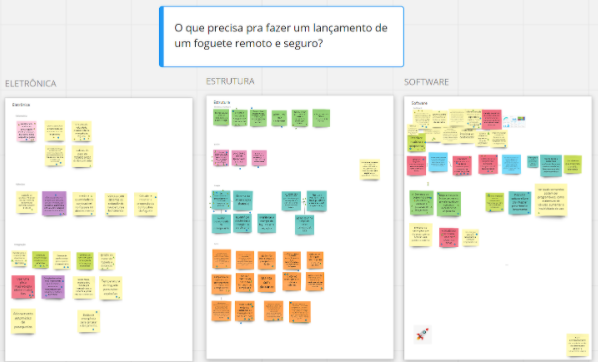
\includegraphics[scale=0.8]{figuras/miro.png}  
\caption{Brainwriting.}
\footnotesize Pode-se acessar em: \url{https://miro.com/app/board/o9J_kmVCAxA=/}
\label{fig:miro}
\end{figure}

\subsubsubsection{\textit{Storyboard}}
Sob a perspectiva de modelos de desenvolvimento, já é comum o uso de histórias de usuários como um aspecto fundamental quando se trata de adotar o modelo \textit{eXtreme Programming}. A ideia consiste em fornecer uma visão de alto nível dos requisitos de um sistema, usadas como principal entrada de informações sobre estimativas e cronogramas, além de guiar a identificação de tarefas de desenvolvimento e conjunto de testes de aceitação (AMBLER, 2004). 

O \textit{storytelling} geralmente concentra-se em três linhas de pesquisas distintas: Geração, Interação ou Visualização das histórias (POZZER, 2005). Assim, nesta etapa do trabalho, a ênfase será na linha de construção que remete a forma como a história é gerada, ou seja, como se dá a elaboração da estrutura que irá guiar aspectos mais gerais, como personagens, ações, objetos e relacionamentos entre usuário e desenvolvedor para que essas especificações sejam geradas.

\textit{Storytelling} é um novo paradigma de entretenimento digital que está avançando a passos largos, com a criação de técnicas e ferramentas que permitem que histórias interativas possam ser criadas, visualizadas e guiadas com o auxílio do computador (POZZER, 2005).
Por fim, a “Exibição” trata a forma de representação gráfica da história, ou seja, a transformação das abstrações das estruturas internas dos personagens em ações realistas dentro de um espaço gráfico.

Contudo, \textit{storytelling} é mais do que um método baseado no ato de contar uma história. Tem como finalidade a captura e a transmissão de conhecimento de forma estruturada. A metodologia adotada pela equipe entrelaça conceitos de RUP e ágil, o que faz que o dinamismo e a relação com o \textit{stakeholder} sejam de fácil acesso e de muita troca de informações, tornando os requisitos mutáveis e adaptáveis à medida que o processo acontece.

Com base nesse contexto, o \textit{storytelling} tem como objetivo assegurar a construção das histórias de usuário com o intuito de prevenir e corrigir as falhas de comunicação e conceito de escopo que possam existir durante o processo.

O artefato que foi gerado pela equipe pode ser conferido abaixo:

"\textit{Guto é um integrante de uma equipe de competição universitária de lançamento de foguetes de pequeno porte e comumente enfrenta problemas com o lançamento dos foguetes da equipe por conta da necessidade da execução manual  obrigatória de rotinas de lançamento.}
    
\textit{Além disso, as informações a respeito do lançamento e do desempenho do foguete são turvas e só podem ser obtidas após a recuperação do foguete, que acontece depois da competição.}

\begin{figure}[H]
\centering
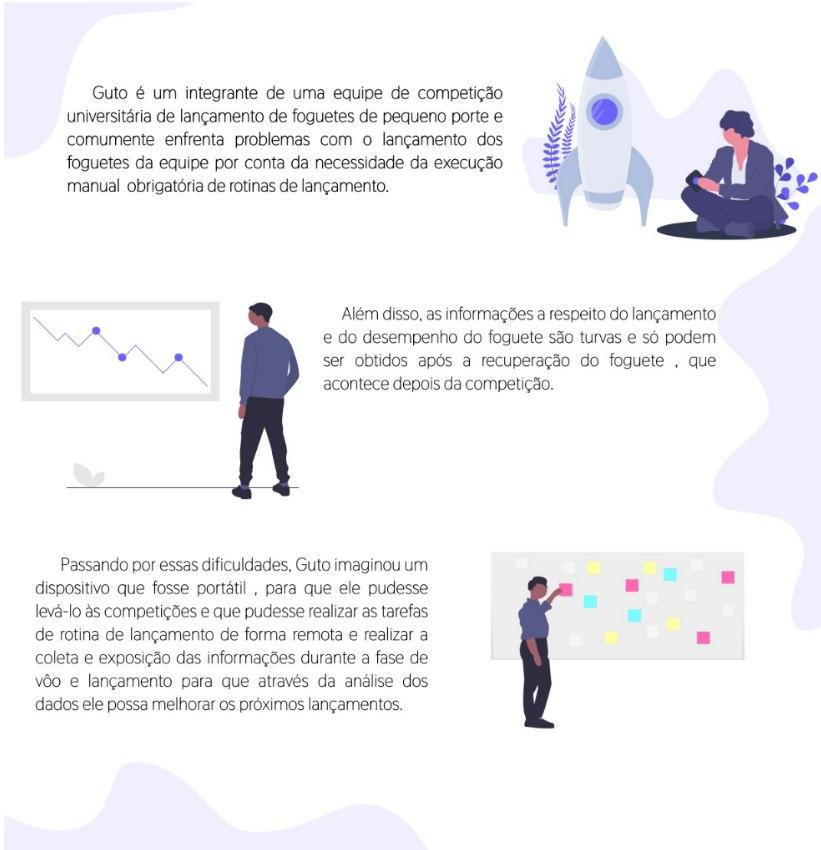
\includegraphics[width=1\textwidth]{figuras/storytelling1.jpg}
\caption{Storytelling, página 1}
\label{fig:storytelling}
\end{figure}

\textit{Passando por essas dificuldades, Guto imaginou um dispositivo que fosse portátil, para que ele pudesse levá-lo às competições, e que pudesse realizar as tarefas de rotina de lançamento de forma remota e realizar a coleta e exposição das informações durante a fase de vôo e lançamento para que através da análise dos dados ele possa melhorar os próximos lançamentos.}

\textit{Assim surgiu o  GCS , um dispositivo portátil, que, além de sanar as dificuldades de Guto, é portátil, seguro, e projetado por meio do método “user centered design”, para que as suas funcionalidades sejam intuitivas e de fácil usabilidade para o usuário.}

\begin{figure}[H]
\centering
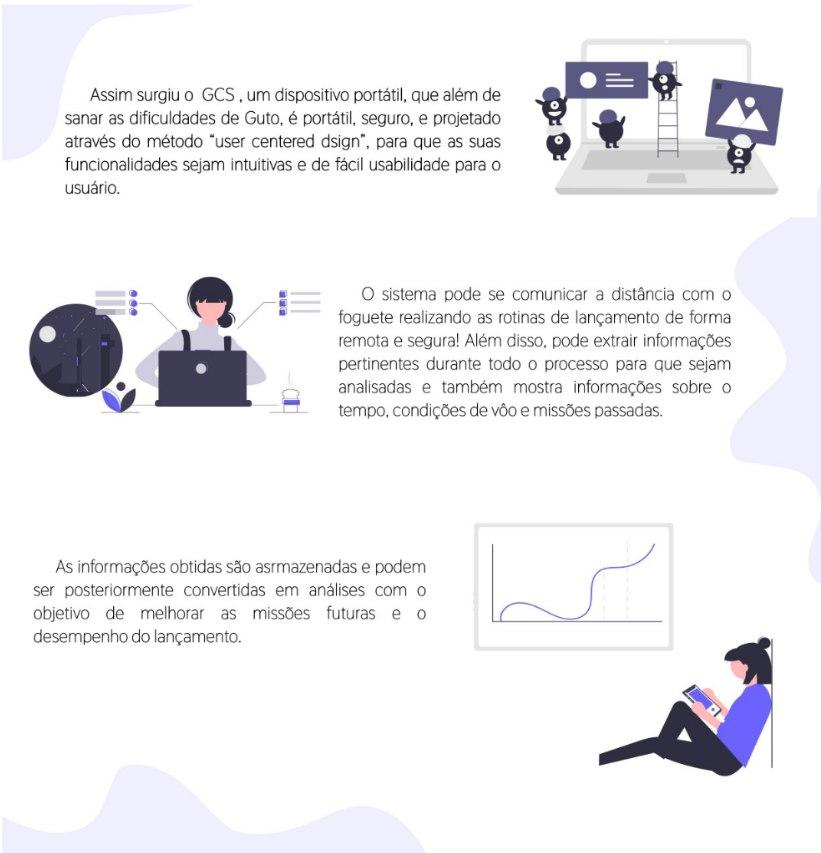
\includegraphics[width=0.9\textwidth]{figuras/sotytelling2.jpg}
\caption{Storytelling, página 2}
\label{fig:sistema de alimentacao}
\end{figure}

\textit{O sistema pode-se comunicar à distância, com o foguete realizando as rotinas de lançamento de forma remota e segura! Além disso, pode extrair informações pertinentes durante todo o processo para que sejam analisadas e também mostra informações sobre o tempo, condições de voo e missões passadas.}"

\subsubsection{Arquitetura da informação}

A arquitetura da informação é a ciência de organizar e categorizar \textit{web sites}, intranets, comunidades \textit{online} e \textit{softwares}, para favorecer a usabilidade e a facilidade, para se encontrar o que se procura \cite{de2011fundamentos}. Ou seja, é a estruturação de toda a informação disponível em um site ou aplicação, para que os usuários possam encontrar fácil e rapidamente o que procuram. E o arquiteto de informação é, na essência, o responsável por isso \cite{de2011fundamentos}. 

Durante a execução desta etapa do projeto, a equipe dedicou-se a executar atividades que fossem relacionadas aos princípios do \textit{User Centered Design}, e, com base nisso, à elaboração de artefatos que ajudassem a construir uma interface intuitiva para o usuário. Os artefatos elaborados pela equipe podem ser conferidos nas sessões seguintes.

\subsubsubsection{\textit{Wireframe}}

Os \textit{wireframes} são diagramas de baixa fidelidade que representam o layout de um site ou aplicação. A sua relevância no processo de \textit{design} deve‐se ao fato de permitirem explorar, testar e iterar ideias de \textit{design} numa fase inicial do projeto, momento em que as mudanças não vão aumentar o orçamento do trabalho. É importante que as pessoas responsáveis pela criação de conteúdo estejam envolvidas no processo de \textit{wireframing} \cite{brito2016usabilidade}. 

Com o objetivo de testar as possíveis versões da interface e iterar a organização estrutural da informação da aplicação, a equipe elaborou um \textit{wireframe}, que foi validado com os usuários e \textit{stakeholders}. Esse artefato pode ser visualizado abaixo.

\href{https://bit.ly/3jnLnmN}{Wireframe}.

\begin{figure}[H]
\centering
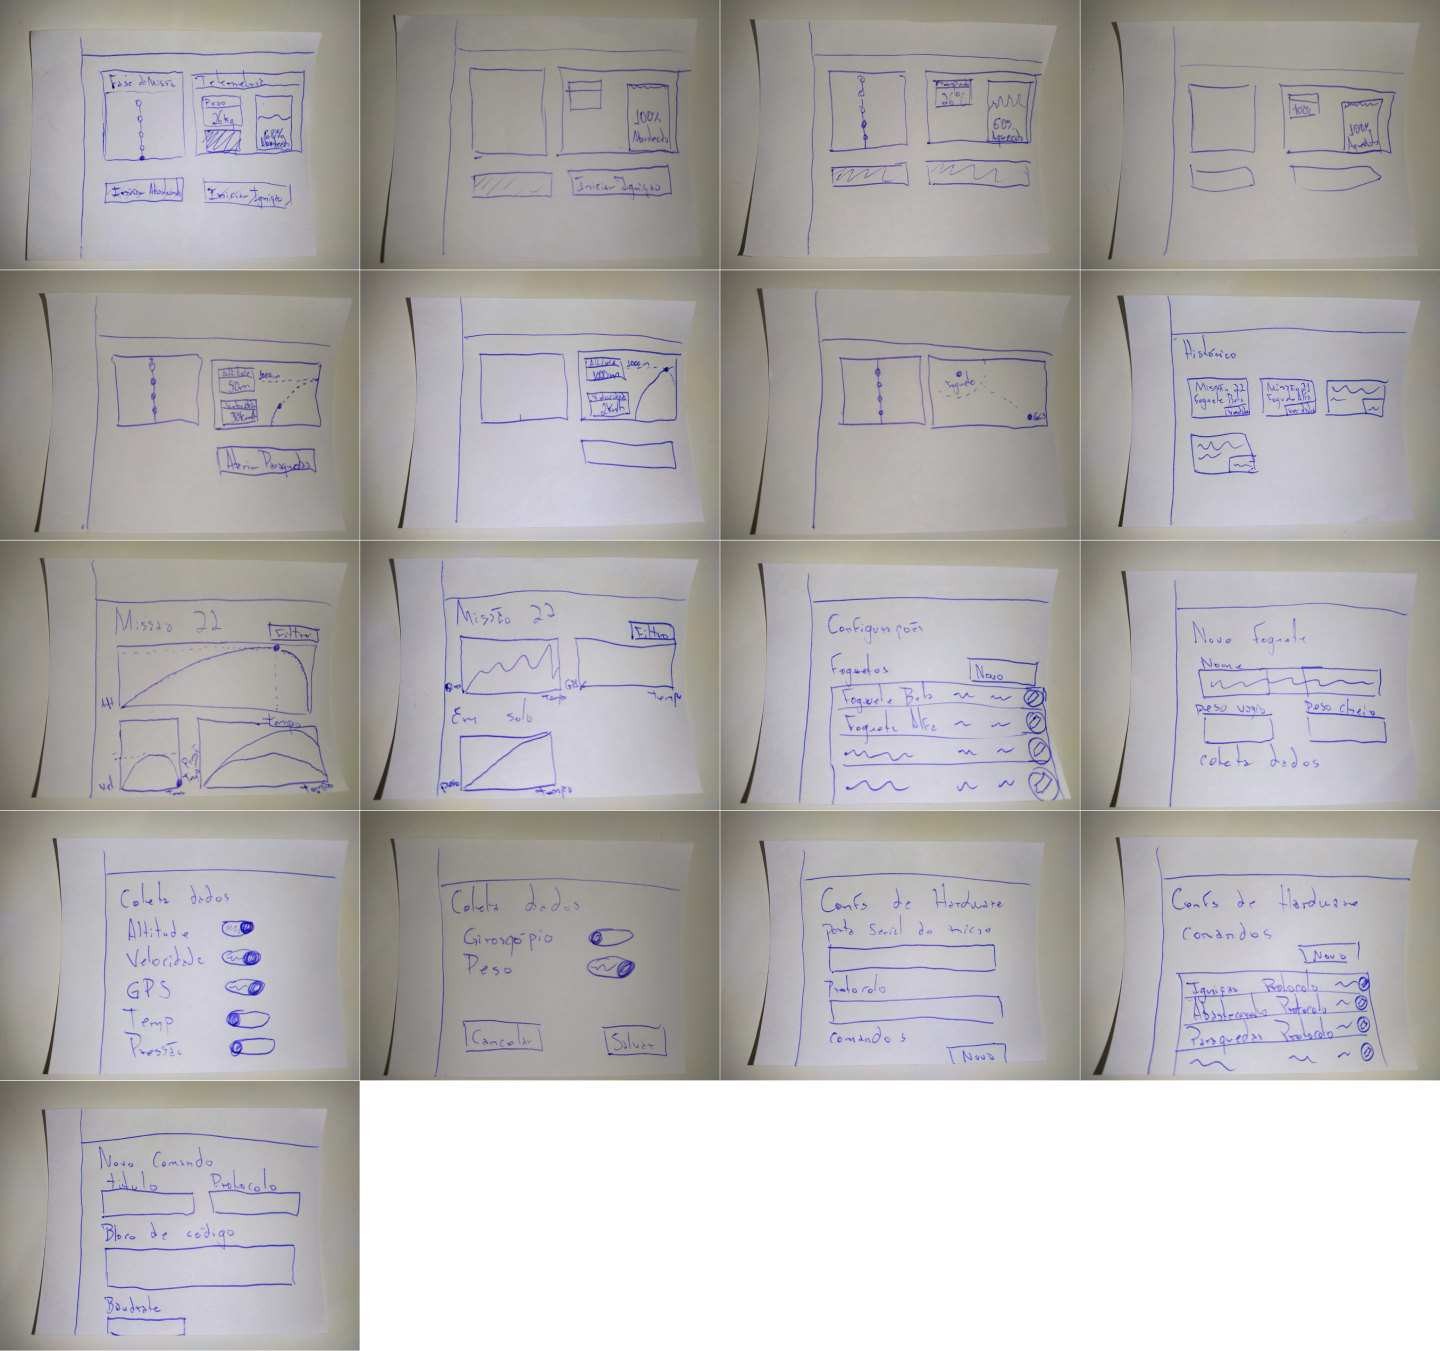
\includegraphics[scale=0.2]{figuras/wireframe.png}  
\caption{Wireframe}
\footnotesize Pode-se acessar em: \url{https://bit.ly/3jnLnmN}
\label{fig:Wireframe}
\end{figure}

\subsubsubsection{Protótipo de média fidelidade}

A prototipação no desenvolvimento de \textit{software} é um processo que tem como função avaliar as ideias geradas e validar – ou não – todos os requisitos estabelecidos \cite{lilley2004development}. É nesse momento que a equipe tende a  tirar as ideias do papel e passar a entendê-las na forma física.

Essa etapa é importante para verificar se a solução desenhada está adequada ao desafio que o cliente enfrenta, garantindo o alinhamento das informações.Dessa forma, conseguimos minimizar os riscos, permitindo que o cliente valide e faça todos os testes antes da implantação. É importante ressaltar que a fase de prototipação pode – e muitas vezes deve – ser realizada em diversos momentos, já que se verificam falhas de forma ágil, chegando assim a uma solução de software mais assertiva.

Apesar de já serem definidos diversos requisitos antes do desenvolvimento do \textit{software}, é durante a interação real do usuário com o sistema que os novos detalhes são percebidos. Para isso, a equipe realizou a elaboração de protótipos de baixa e média fidelidade, com a colaboração dos usuários e \textit{stakeholders}. As versões dos protótipos podem ser conferidas a seguir:


\href{https://bit.ly/35xe23N}{Protótipo V0}.

\href{https://bit.ly/2FW3oep}{Protótipo V1}.

\href{https://bit.ly/34pAfS2}{Protótipo V2}.

\subsubsection{Definição do produto}

O projeto aplica-se a um contexto de competições de lançamento de foguetes experimentais, onde cada equipe constrói seu foguete com base no regulamento da competição. Os projetos necessitam estar adequados o melhor possível às regras para obter uma boa pontuação. Devido à dinamicidade dos projetos e da baixa restrição de \textit{hardware} das competições, temos diversas configurações de \textit{hardware}. Nesse contexto, os sistemas de \textit{software} têm uma grande necessidade de adequação e adaptação aos diferentes \textit{hardwares} possíveis.

O produto de \textit{software} visa auxiliar o controle e monitoramento do lançamento de um foguete experimental para competições, provendo segurança, controle e visão de uma missão\footnote{Uma missão é todo o processo de lançamento de um foguete em uma competição. Vai desde a preparação para o abastecimento até a coleta do foguete após pousar.}. O sistema irá atuar em 3 momentos na competição:
\begin{itemize}
    \item abastecimento e ignição do foguete;
    \item foguete em voo;
    \item foguete em pouso.
\end{itemize}

Em ambos os momentos da competição, o sistema comunicar-se-á com \textit{hardwares} externos para fazer as leituras e enviar comandos de controles. 
Para tornar o produto de software valioso para os clientes, é fundamental satisfazer os objetivos e restrições expostos. Assim, faz-se necessária a construção de um sistema que permita a visualização e controle dos processos da missão, a partir de dados de telemetria e comandos para o \textit{hardware}, sendo estes configuráveis.Portanto, podemos definir as principais funcionalidades do sistema como:
\begin{itemize}
    \item possibilitar a leitura e exposição dos dados de telemetria do foguete:
    \begin{itemize}
        \item GPS;
        \item Altitude;
        \item Velocidade;
        \item Temperatura;
        \item Pressão;
        \item Giroscópio;
        \item Peso (em solo); 
    \end{itemize}
    \item possibilitar comandos de ignição, abastecimento e abertura do paraquedas;
    \item possibilitar configuração dos comandos e protocolos necessários para se comunicar com diferentes \textit{hardwares};
    \item armazenar os dados de maneira segura.
\end{itemize}

\subsubsubsection{Mapa de requisitos}

\begin{figure}[h!]
\centering
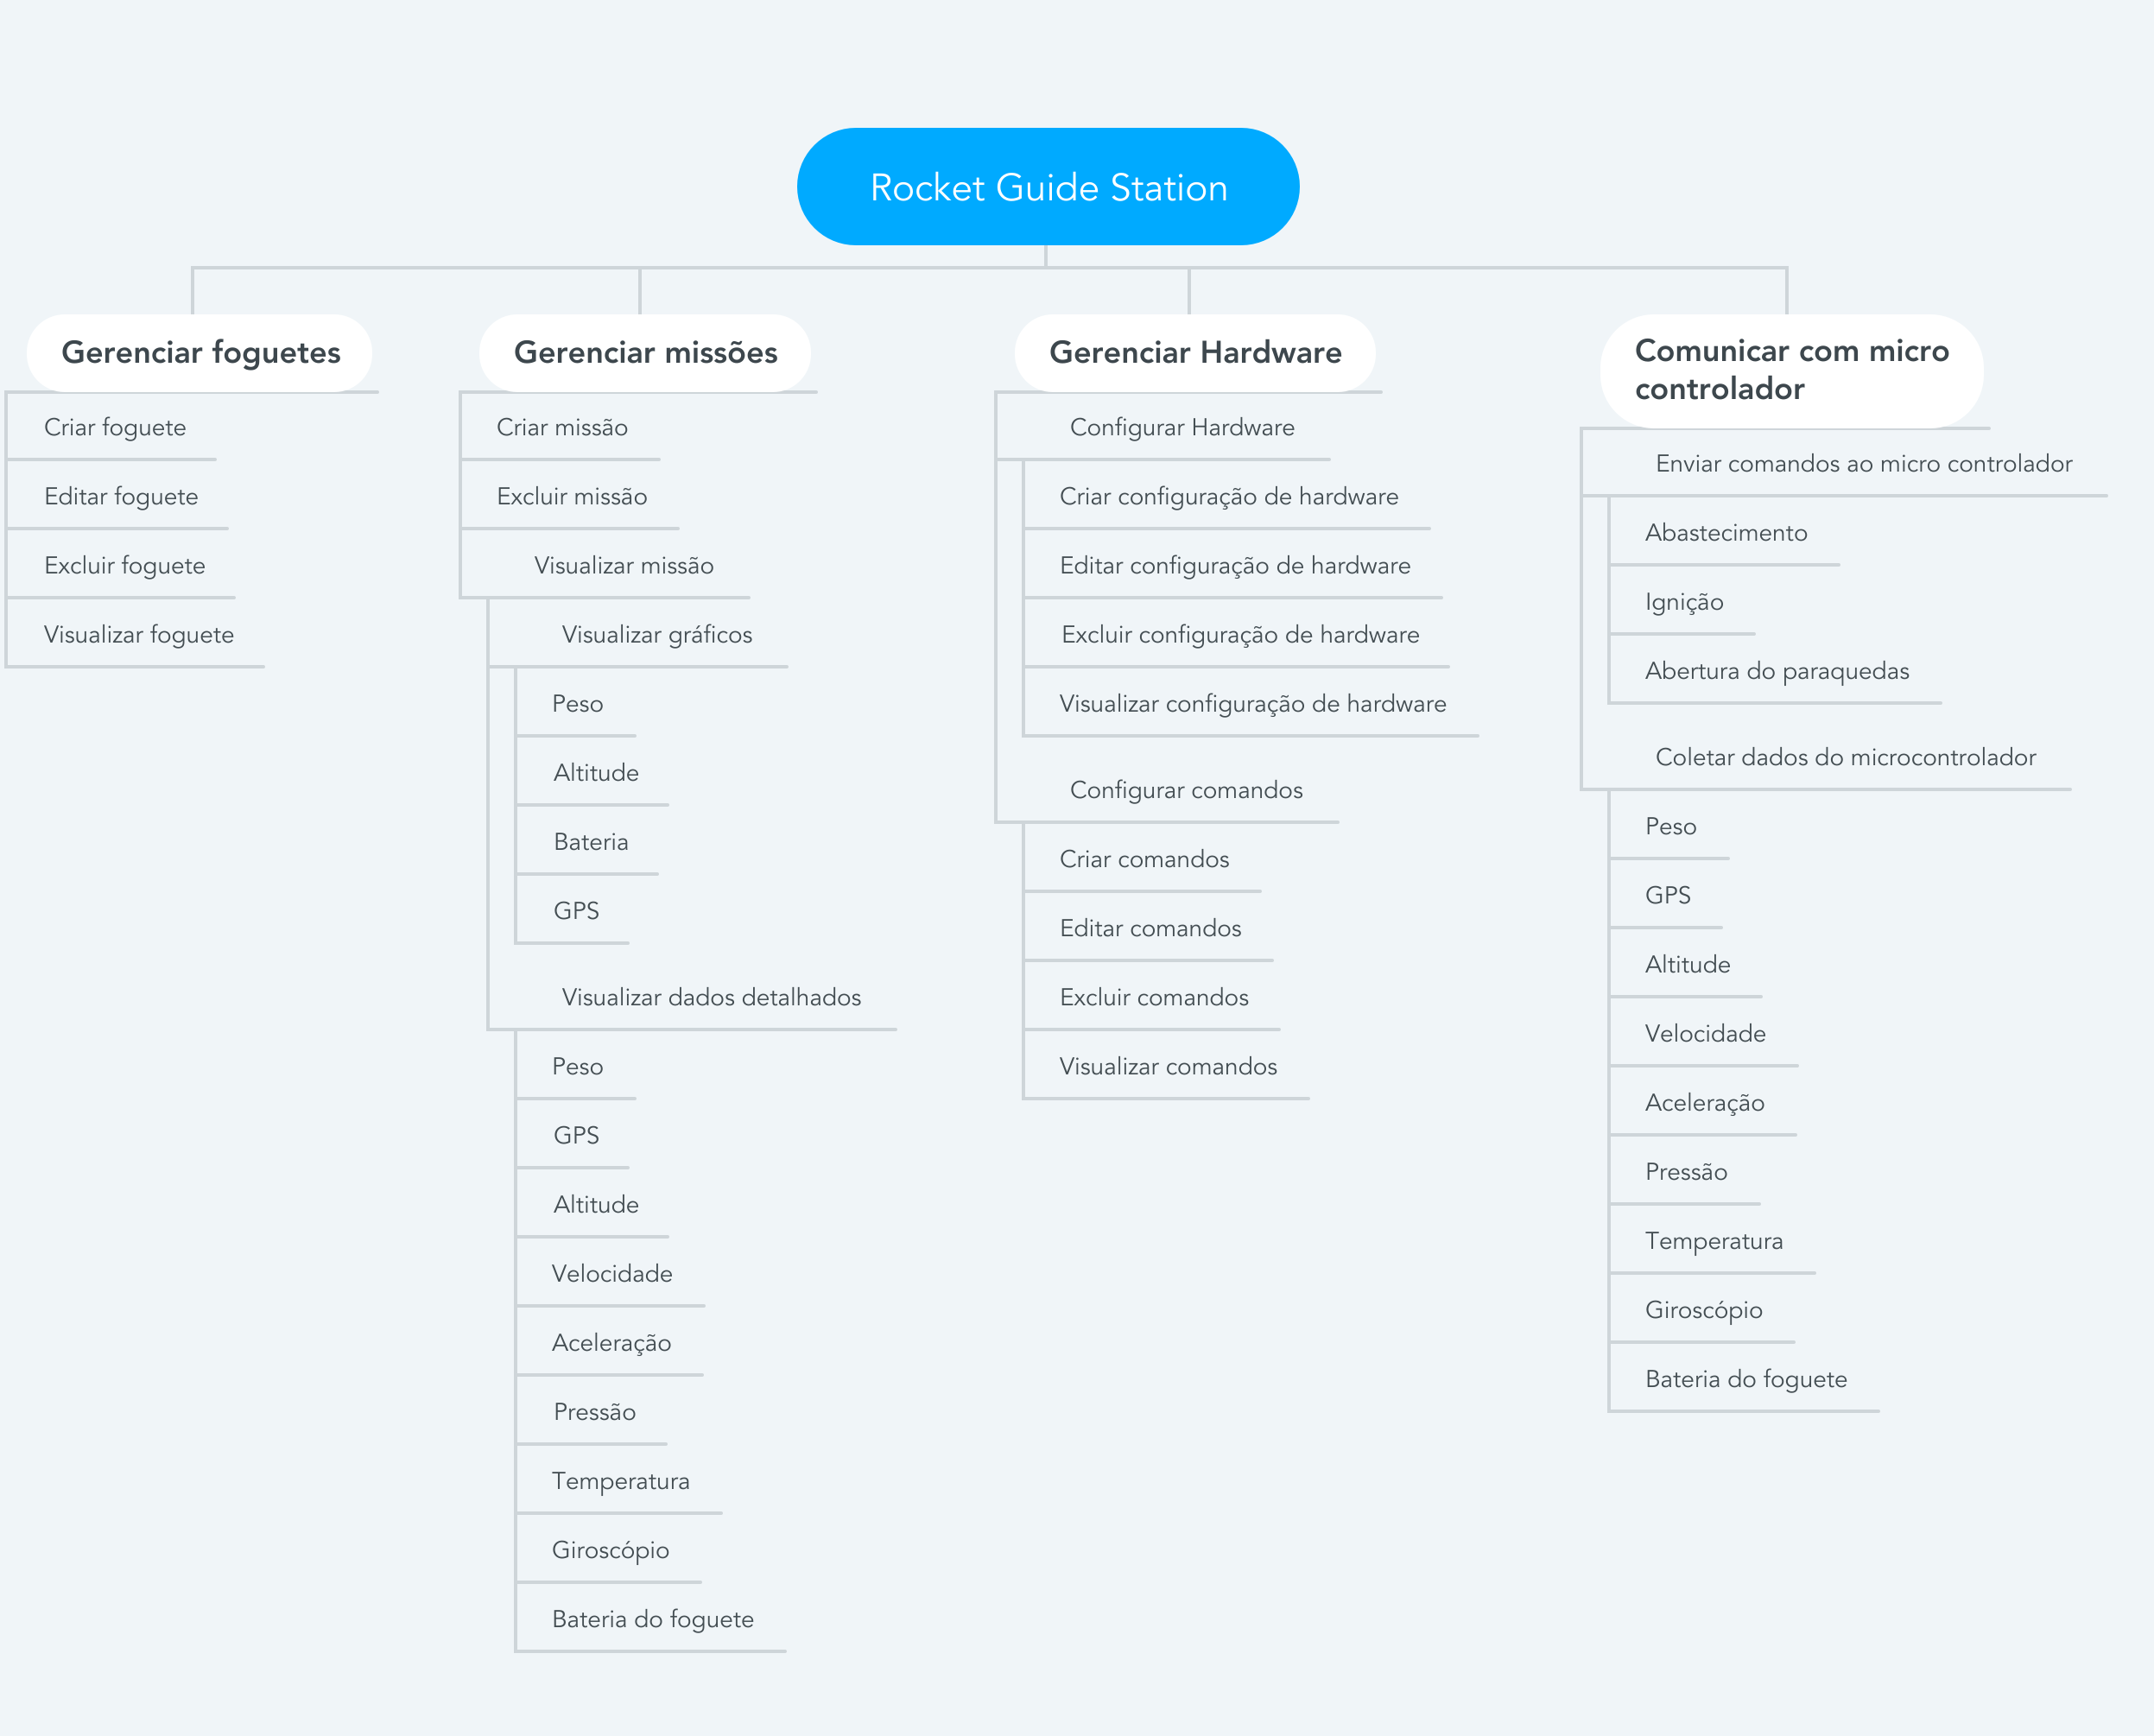
\includegraphics[scale=0.15]{figuras/Rocket_Guide_Station.png}  
\caption{Mapa de requisitos}
\label{fig:Mindmeister}
\end{figure}

Neste projeto, aplicamos técnicas de mapa mental para fazer a especificações de requisitos \cite{mapamental}. Utilizamos a ferramenta \textbf{Mind Meister} para construir o mapa mental.
A partir da nova definição de produto, foi feito um mapa de requisitos demonstrando todos os requisitos do projeto. A Figura \ref{fig:Mindmeister} apresenta os épicos, ou principais funcionalidades: \textbf{Gerenciar Foguetes}; \textbf{Gerenciar Missões}; \textbf{Gerenciar Hardware}; e \textbf{Comunicar com o Micro Controlador}. Essas informações também estão disponíveis no link à seguir:  (https://mm.tt/1664123184?t=VJwmqWSqXf).



\subsection{Problemas na Solução Antiga}
\label{problema_solucao_antiga}
Antes de criar ou implantar uma \textit{feature} de \textit{machine learning}, deve-se levar em consideração alguns pontos cruciais para a criação e especificação do produto. Desenvolver um produto de \textit{Machine Learning} (ML) demanda um processo mais complexo e requer mais processamento de \textit{hardware}. Portanto, levamos em consideração algumas ponderações sobre as necessidades do cliente e quais as melhores soluções a serem adotadas e, por fim, verificar a necessidade de utilizar ML para resolver esse problema \cite{shams2018developing}.

Primeiro, entendemos que, em um clássico programa, é necessário especificar as regras sobre o que deverá ser feito. Já para ser necessário aplicar ML, essas regras são tantas que não são escaláveis para resolver em um produto comum. A utilização de um algoritmo ou do poder de ML dá-se quando as regras não são precisas ou não são conhecidas, mas temos muitos dados e respostas. Consequentemente, para desenvolver esse produto, é necessário ter um grande problema a ser resolvido, com muitas regras desconhecidas (tantas que se torna difícil implementar usando um software comum) \cite{amershi2019software}. Quando se deseja desenvolver um produto, é necessário ter em mente duas coisas principais:
\begin{itemize}
    \item qual o problema a ser resolvido e quais as respostas esperadas?
    \item temos acesso a muitos dados?
\end{itemize}

Se conseguimos responder corretamente essas duas questões, desenvolver um produto de ML é a melhor solução. Nesse projeto, a primeira questão é facilmente respondida, mas a quantidade de dados e informações inviabiliza o desenvolvimento de um ML, pois o produto de ML é um ciclo, onde no início de tudo, é utilizado \textbf{dados}, com esses dados conseguimos fazer boas \textbf{predições}. Essas predições melhoram a \textbf{experiência do cliente}, que acabam gerando mais \textbf{tráfego} e utilização, que implica em ter mais dados e consequentemente mais informações \cite{yandong2005development}. A falta de dados para iniciar esse processo, inviabiliza a utilização desse tipo de solução nesse projeto.

Existem outros quatro fatores importantes que foram levados em consideração na concepção e \textit{design} desse produto:

\begin{itemize}
    \item \textbf{Lógica muito complexa:} A necessidade dos clientes desse projeto, não possui uma lógica complexa a ponto de não ser possível resolver com um software comum. As regras são conhecidas e facilmente manipuladas.
    
    \item \textbf{Rápida escalabilidade:} Esse projeto possui um problema complexo, mas é um problema pequeno, não possui muitos dados complexos e a utilização não é tão frequente quanto o necessário para utilizar ML. (ex: O Diário Oficial é publicado diariamente, às vezes até mais uma vez por dia, e possui uma série de informações diferentes em cada um, portanto este é um exemplo de problema que necessita de uma rápida escalabilidade).
    
    \item \textbf{Requer personalização especializada:} Uma das vantagens de utilizar ML é o seu poder de identificar padrões e regras específicas de cada necessidade em um cenário com inúmeras necessidades. Neste projeto as necessidades são mensuráveis e poucas especificidades relacionadas à elas.
    
    \item \textbf{Adaptação em tempo real:} Por último e não menos importante, é importante verificar se o problema identificado hoje poderá ser modificado no futuro. Neste projeto, identificamos que as necessidades podem ser modificadas de acordo com os componentes de \textit{hardware} e sensor, o edital e as regras da competição, portanto é um problema que necessita de uma adaptação em tempo real.
\end{itemize}

Após analisar esses pontos, entendemos que a solução desse projeto não precisa ser - e de fato não é recomendado que seja - resolvida com o uso de ML. Ao primeiro momento, o objetivo será focar em coletar e iniciar o armazenamento de dados para que futuramente possa ser inserido uma \textit{feature} de ML para resolver problemas mais complexos. A implantação de um ML no projeto no momento atual não se faz necessária e tem alto custo de processamento. Ela pode atender as necessidades do cliente, mas é uma ferramenta muito poderosa para ser aplicado no problema atual.


\subsection{Definição da Arquitetura}


%https://miro.com/app/board/o9J_kiYMRcI=/

\subsubsection{Padrão Arquitetural}
De acordo com o problema que o projeto visa resolver, a solução técnica proposta será embasada na arquitetura REST. A arquitetura \textit{Representational State Transfer} (REST), em português Transferência Representacional de Estado, é ideal ao nosso sistema, pois ele possui baixa complexidade e necessidade de utilização dos dados em tempo e estado definidos. De acordo com (TRIPOLI; CARVALHO, 2016) em suas conclusões, um sistema nem sempre se encaixa no perfil de um arquitetura distribuída, como a arquitetura micros-serviços, que, se aplicada de modo equivocado, pode prejudicar o bom andamento do projeto, pois exige maior complexidade no desenvolvimento e implantação do sistema, concluindo que esse tipo de arquitetura não deve ser aplicada a \textit{softwares} simples e com baixo grau de complexidade. 

A complexidade de um sistema nada diz sobre a eficiência e eficácia deste. Nossa solução proverá uma comunicação necessária para que as regras de negócio sejam aplicadas, satisfazendo as expectativas dos usuários e clientes. Após um estudo, foi verificado que uma \textit{Application Programming Interface} (API), em português Interface de Programação de Aplicativos, que seja RESTful, ou seja, capaz de implementar a arquitetura REST, é ideal para o problema proposto. 

No diagrama com protocolos de comunicação entre componentes do software Figura 8, vemos que a comunicação entre os componentes do sistema deve ser planejada de maneira sistemática, e esse foi o caso. O sistema será construído usando a linguagem de programação JavaScript. O uso de JavaScript é bem comum para os \textit{browsers}, porém é necessários ajustes para a sua utilização a nível de \textit{backend}. Esses ajustes são realizados pelo \textit{runtime} Node.js, um ambiente em tempo de execução capaz de rodar um servidor \textit{web} local na porta 4200 como padrão. O Node.js, além de permitir a execução de código localmente fora no navegador, é responsável também por gerenciar pacotes e empacotar tudo que é necessário para executar e interpretar código JavaScript.

Na Figura \ref{fig:javascript backend} \cite{javascript-backend} vemos a lógica por trás da aplicação da linguagem JavaScript em nossa API.

\begin{figure}[h!]
	\centering
	\label{javascript backend}
		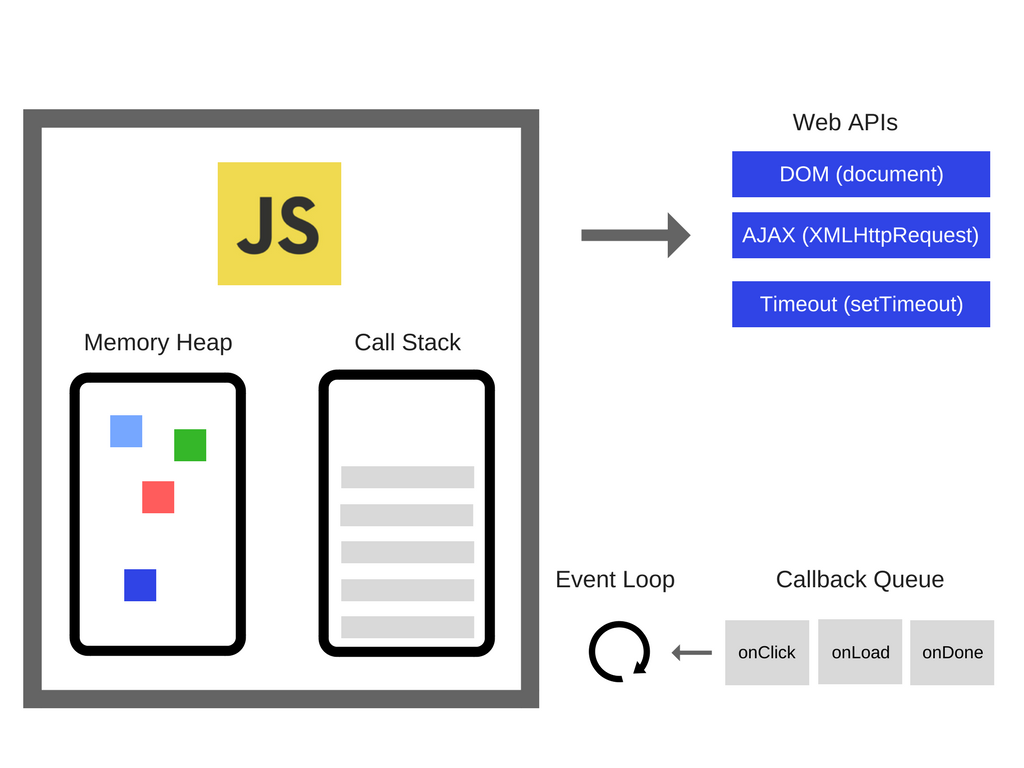
\includegraphics[keepaspectratio=true,scale=0.5]{figuras/javascript-backend.png}
	\caption{Modo como o JavaScript é executado fora do browser}
	{\footnotesize Fonte: \cite{javascript-backend}}
	\label{fig:javascript backend}
\end{figure}



\subsubsection{Representação da Arquitetura}

\begin{figure}[H]
\centering
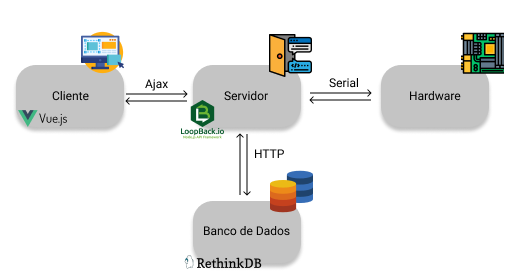
\includegraphics[width=0.9\textwidth]{figuras/representacao_arq.png}
\caption{Representação da Arquitetura}
\label{fig:representacao_arq}
\end{figure}


\subsubsubsection{Cliente}

Em aplicações \textit{web}, é muito comum adotar o conceito de \textit{Client-side} e \textit{Server-side} dentro da arquitetura em camadas \cite{ServerAndClient}. Nossa aplicação não será essencialmente \textit{web}, já que não será possível executar um \textit{browser} e também ter acesso à internet, assim como citado na Seção \ref{metas_restricoes} deste documento. Porém, vamos usar uma tecnologia inovadora implementada pelo \textit{framework} JavaScript Electron.js, que possibilita o desenvolvimento de aplicações \textit{desktop cross-platform}, em português seria algo como uma mescla de tipos de plataformas (\textit{web} e \textit{desktop}), utilizando ferramentas \textit{web} como JavaScript, HTML e CSS \cite{electron}.

O ciclo de vida do lado do Cliente (\textit{Client-side}) é representado na figura \ref{fig:client-side}. O JavaScript faz requisições, ações que o usuário deseja executar ao utilizar a interface da aplicação, por meio de chamadas AJAX (Asynchronous JavaScript And XML), em português seria algo como JavaScript assíncrono + XML \cite{Ajax}. Com essa tecnologia, uma aplicação \textit{web} é capaz de realizar atualizações incrementais na interface apresentada ao usuário.

\begin{figure}[!h]
	\centering
		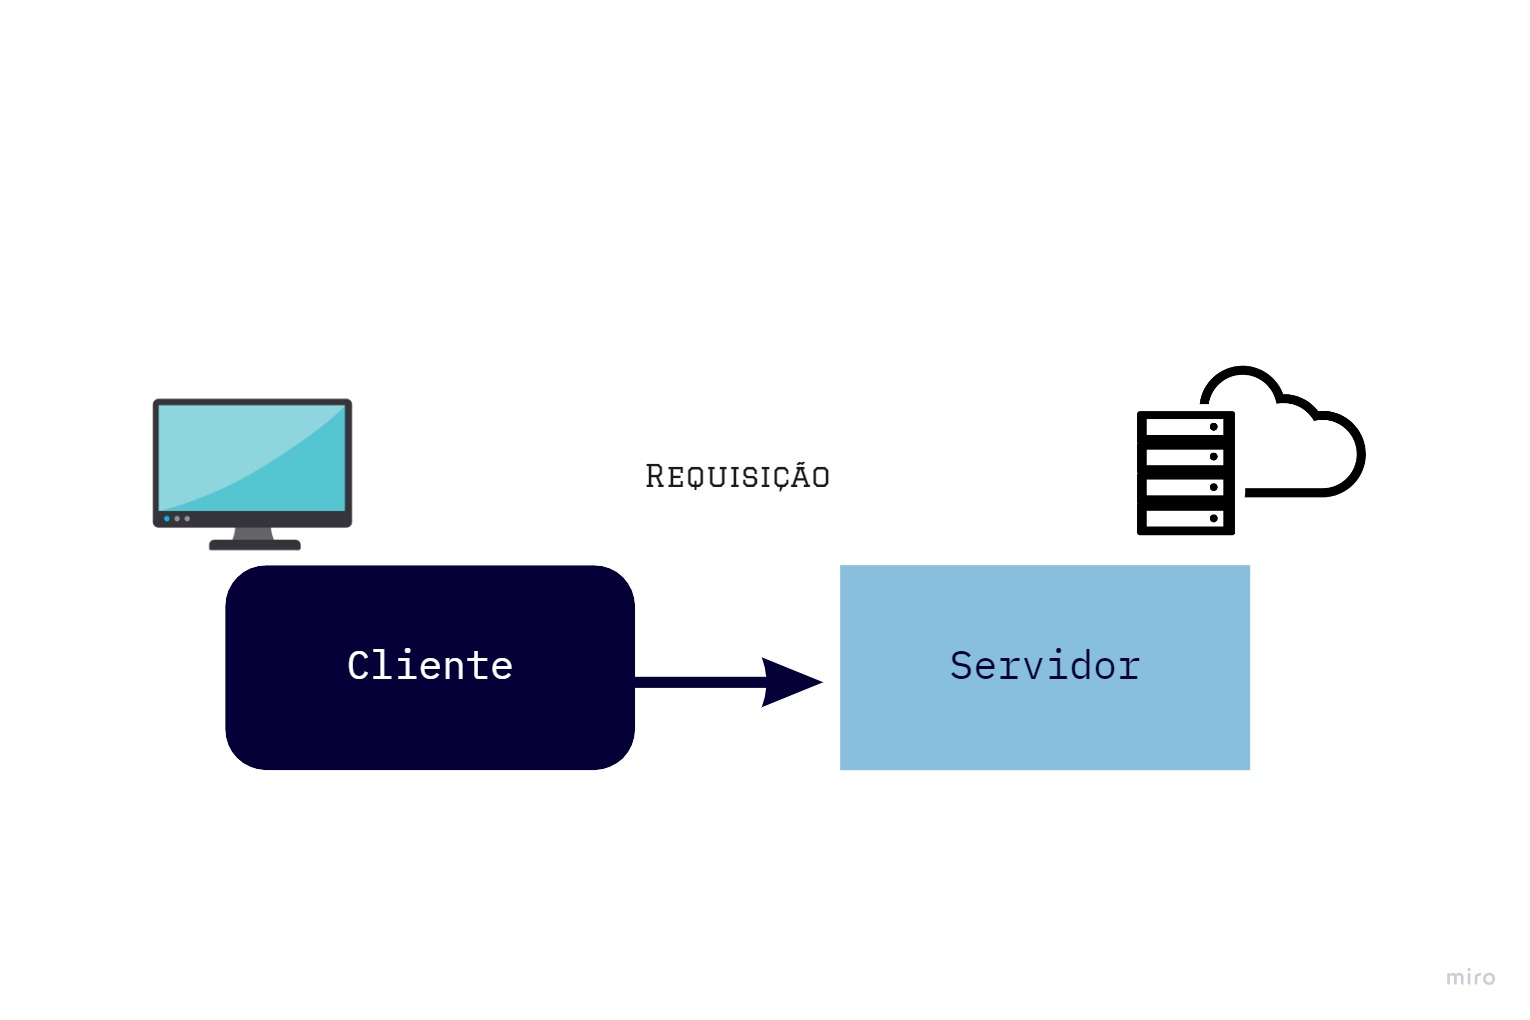
\includegraphics[keepaspectratio=true,scale=0.3]{figuras/client.jpg}
	\caption{Cliente da aplicação Desktop}
	\label{fig:client-side}
\end{figure}


A tecnologia que será usada é o Vue.js um \textit{progressive framework}, em português "\textit{framework} progressivo", em JavaScript para o desenvolvimento no \textit{Client-side} \cite{Vue} e também fazendo uso do "axios" que é um cliente HTTP baseado em \textit{promises}, que é um objeto usado para processamento assíncrono \cite{Promise}. Nesse contexto, o desenvolvimento \textit{frontend} será responsável por criar a interface gráfica e também a comunicação entre \textit{Client-side} e \textit{Server-side}. 

\subsubsubsection{Servidor}

Do lado do servidor, \textit{Server-side}, temos recebimento de requisições por parte do cliente, o processamento lógico e, por fim, o envio da resposta correspondente ao cliente. 

\begin{figure}[!h]
	\centering
		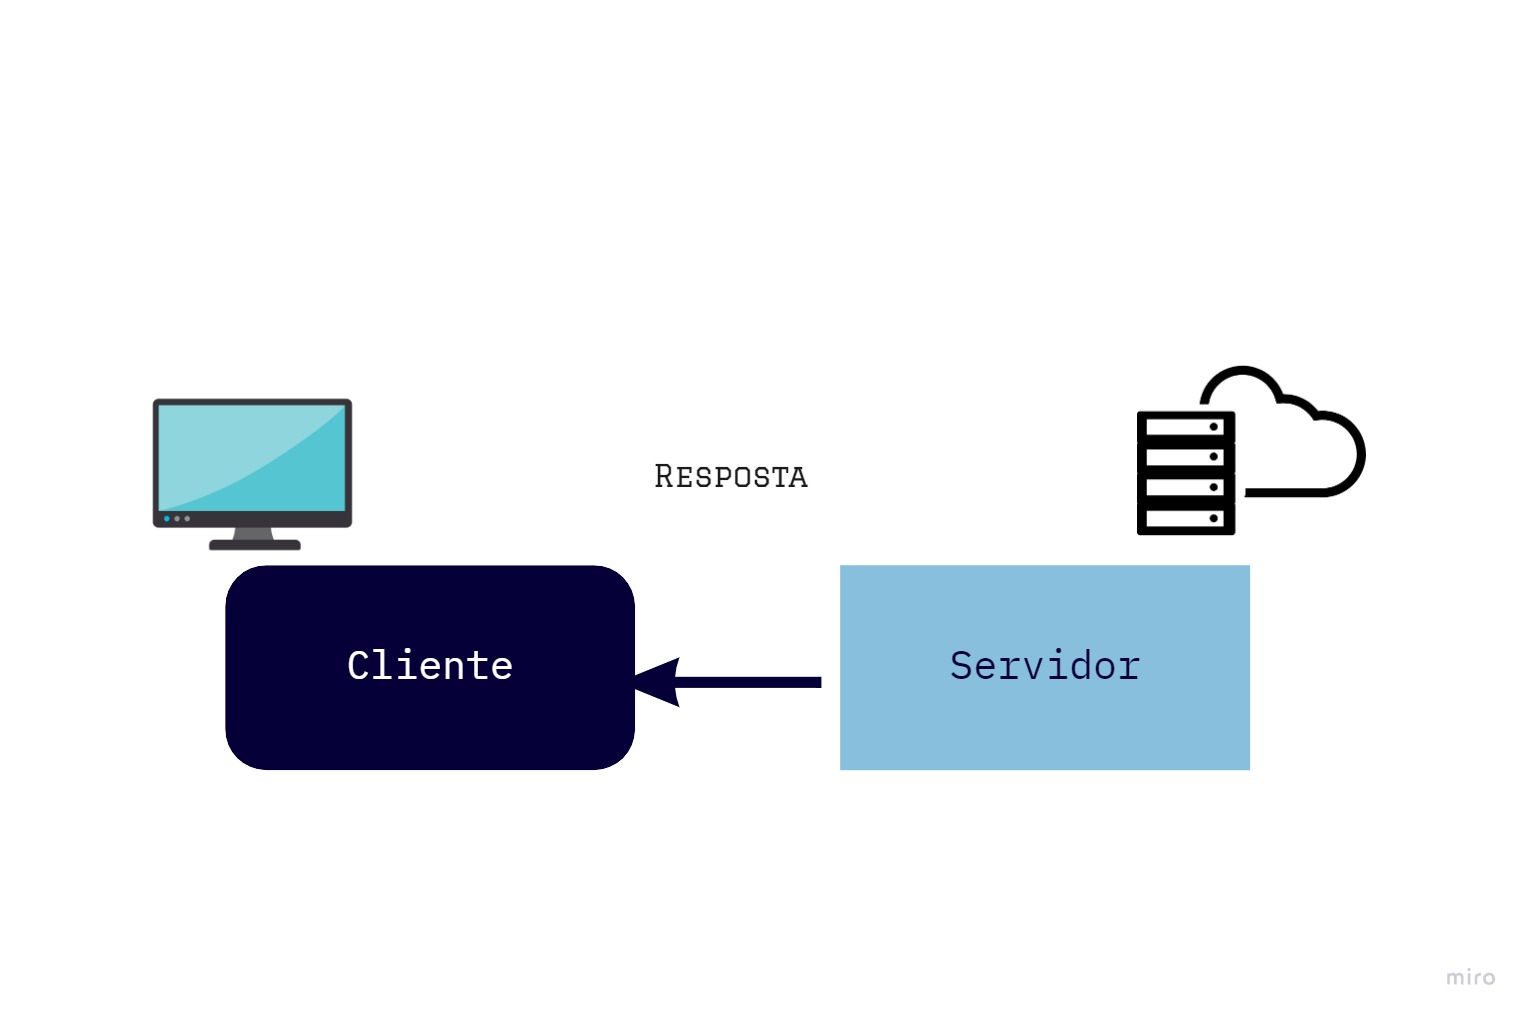
\includegraphics[keepaspectratio=true,scale=0.3]{figuras/server.jpg}
	\caption{Servidor da aplicação Desktop}
	\label{fig:client-side}
\end{figure}

Faremos uso de uma API Rest escrita em JavaSript, por meio do Framework Loopback, um \textit{framework} altamente expansível baseado no famoso Express e em Node.js + Typescript \cite{Loopback}. Dessa forma, poderemos criar serviços REST que serão consumidos pelo Cliente por meio de \textit{endpoints}.

Para o \textit{pipeline} de funções que manipulam as requisições e respostas HTTP que serão necessárias para a comunicação com o Banco de dados, faremos o uso de \textit{middleware}. Esse tipo de metodologia de processamento implementa o padrão de projeto \textit{Chain of Responsability}  \cite{Chain}, o qual é desenhado para desacoplar o envio e recebimento de mensagens dividindo a tarefa de manipulá-las entre múltiplos objetos tal como na figura \ref{fig:chain-of-responsibility}:

\begin{figure}[!h]
	\centering
	\label{chain-of-responsibility}
		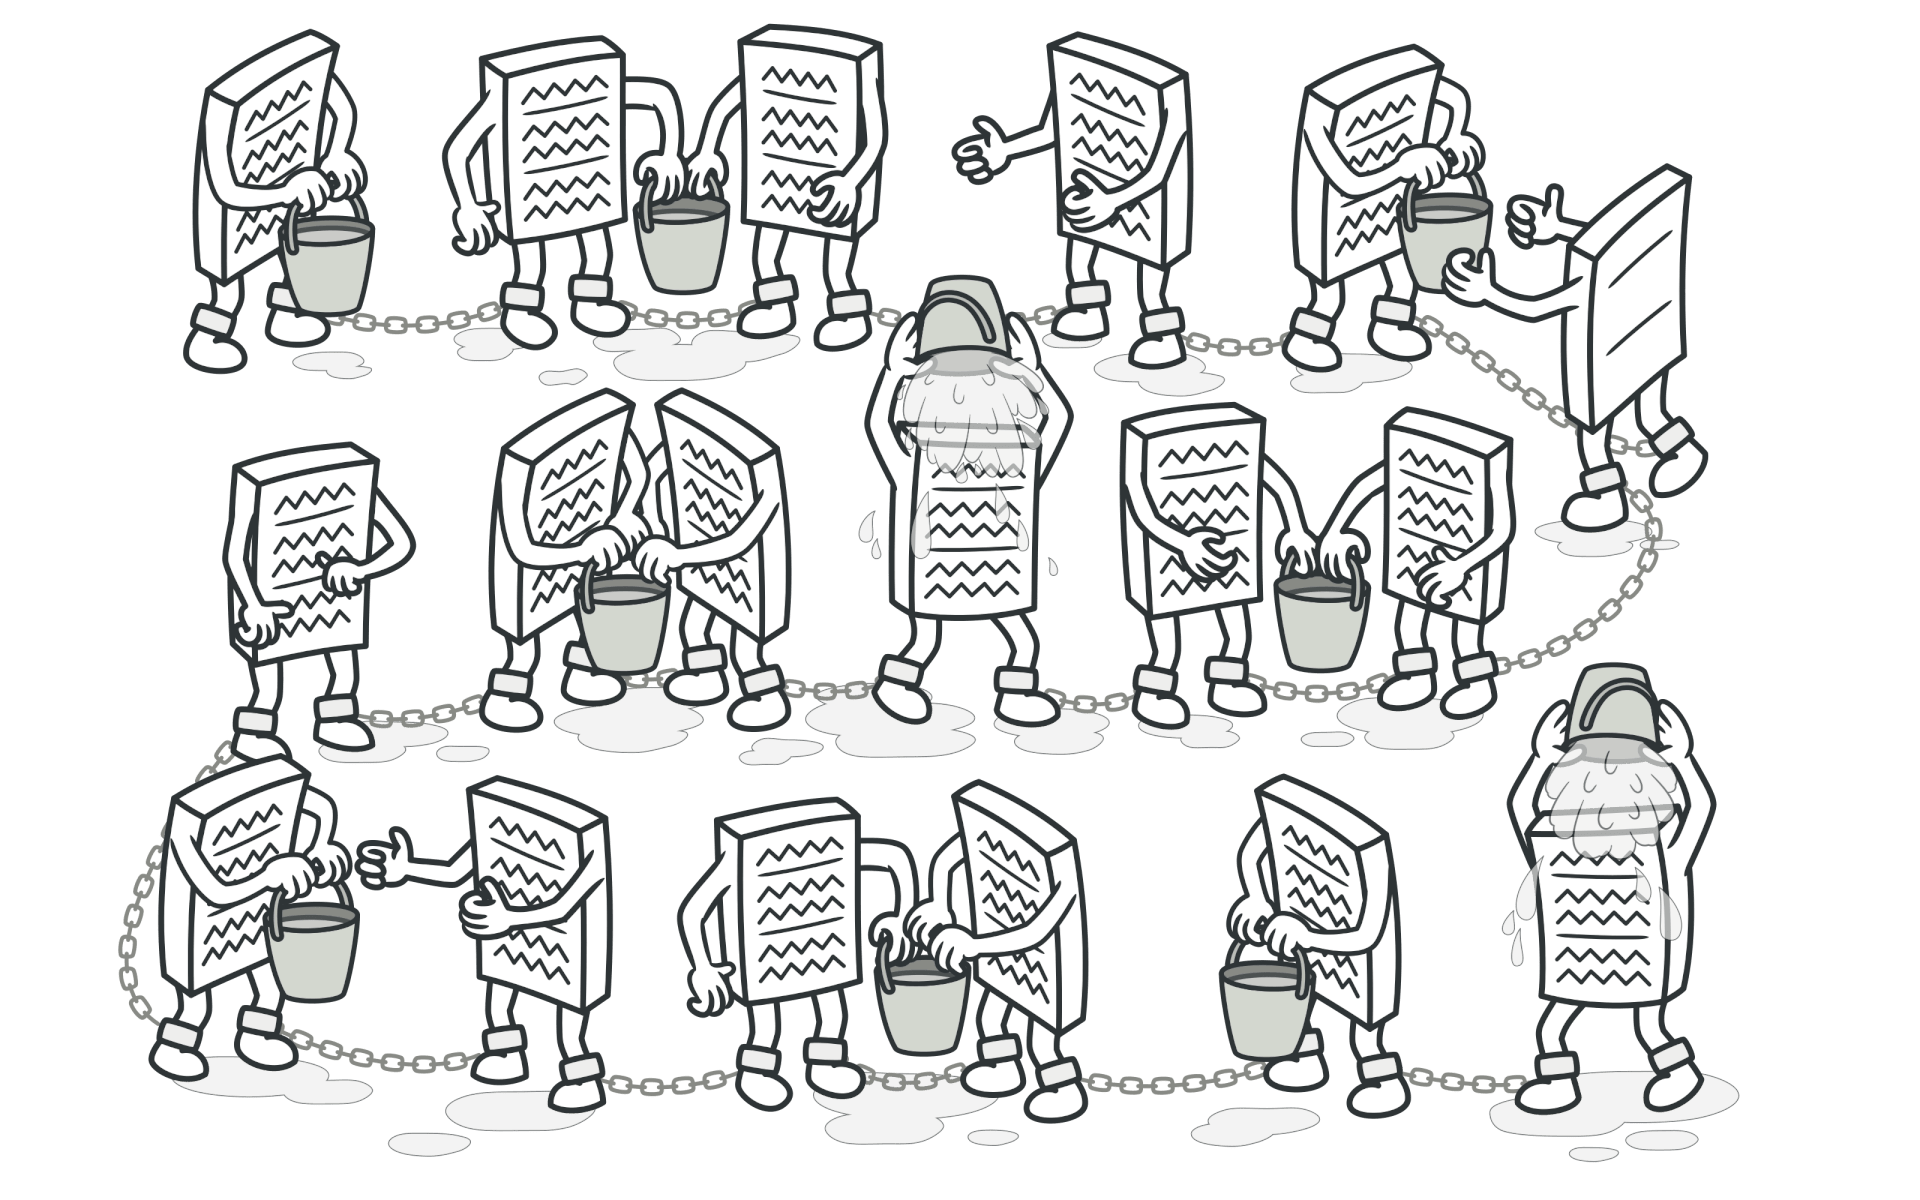
\includegraphics[keepaspectratio=true,scale=0.25]{figuras/chain-of-responsibility.png}
	\caption{Padrão de Projeto Chain of Responsability \cite{ChainFigura}}
	\label{fig:chain-of-responsibility}
\end{figure}

Com o \textit{Loopback}, podemos criar uma sequencia de funções que realizam o processamento adequado de mensagens conforme representado na Figura \ref{fig:middleware} \cite{Loopback}.

\begin{figure}[!h]
	\centering
	\label{middleware}
		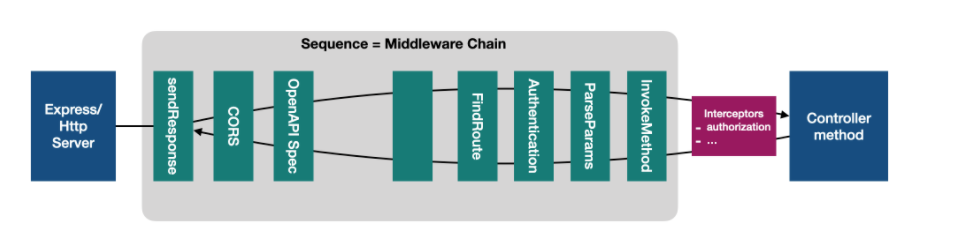
\includegraphics[keepaspectratio=true,scale=0.9]{figuras/middleware.png}
	\caption{Sequência baseada em Middleware  \cite{Loopback}}
	\label{fig:middleware}
\end{figure}


\subsubsubsection{Banco de Dados}

Para oferecer uma experiência satisfatória ao usuário da aplicação, os dados devem ser apresentados em tela em tempo real. Nossa base de dados deve ser capaz de detectar qualquer mudança realizada em seu armazenamento. Para isso, optamos por usar a tecnologia do banco de dados RethinkDB, um banco de dados open-source capaz de realizar envio de dados no formato JSON em tempo real. 
Além disso, é um banco de dados NoSQL, que nos permite flexibilidade se comparado com bancos SQL, mas que mantém a organização a nível de modelagem de dados. A tecnologia por trás disso é a \textit{schemaless JSON documents}, um armazenamentos de documentos JSON não esquematizado.Todos os documentos NoSQL armazenam suportam as mesmas operações básicas:

\begin{itemize}
    \item criar ou apagar registros de uma coleção;
    \item criar, recuperar, atualizar ou deletar um documento;
    \item consultar uma coleção;
    \item criar ou apagar registros de índices. 
\end{itemize}

Dessa forma, teremos uma ferramenta poderosa para manipular nossos dados.Diferentemente de bancos SQL, os arquivos são escritos em documentos, com estruturas semelhantes às abaixo:

\begin{figure}[!h]
	\centering
	\label{json}
		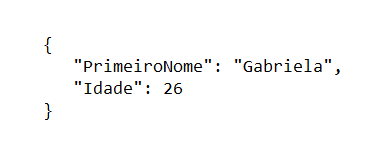
\includegraphics[keepaspectratio=true,scale=0.9]{figuras/json.png}
	\caption{Documento em formato JSON}
	\label{fig:json}
\end{figure}

\begin{figure}[!h]
	\centering
	\label{xml}
		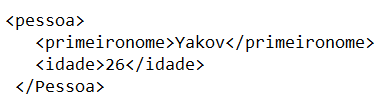
\includegraphics[keepaspectratio=true,scale=0.9]{figuras/xml.png}
	\caption{Documento em formato XML}
	\label{fig:xml}
\end{figure}

\subsubsubsection{\textit{Hardware}}

A comunicação entre o \textit{hardware} e o \textit{software} do projeto é feita via porta serial. Em fase experimental, iremos fazer um \textit{script} para simular o funcionamento dessa integração e relatar o desempenho possível e desejado. Até o momento, não foram encontradas evidências de que o \textit{script} poderá ser escrito em JavaScript, já que existe a biblioteca Serialport.js \cite{serialport} que dá o necessário suporte a esse tipo de comunicação. Porém, caso haja qualquer problema de compatibilidade, faremos uso do padrão de projeto Adaper, que tem como objetivo prover uma interface que liga objetos com diferentes tipos de linguagem e protocolos de comunicação. O padrão é representado pela Figura \ref{fig:adapter}:

\begin{figure}[!h]
	\centering
	\label{adapter}
		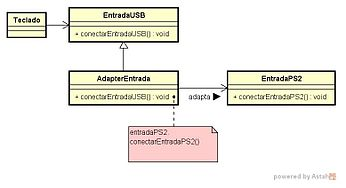
\includegraphics[keepaspectratio=true,scale=1]{figuras/adapter.jpg}
	\caption{Padrão de projeto Adapter \cite{Adapter}}
	\label{fig:adapter}
\end{figure}

\subsubsection{Ambiente}
Tendo em vista a arquitetura do projeto e a falta da placa para testar o sistema nas condições reais, foi adotada a estratégia de conteinerização dos serviços. Assim é possível isolar os ambientes, bem como facilitar a configuração do ambiente de produção (já embarcado no dispositivo). Para isso, foram utilizadas as seguintes tecnologias:

\begin{itemize}
    \item Docker \cite{docker}
    \item Docker - Compose \cite{docker-compose}
\end{itemize}

\subsubsection{Arquitetura computacional}
O sistema será desenvolvido para ser executado em um computador de arquitetura 64 bit ARM (Arm64) e um sistema operacional que opere nessa mesma arquitetura \cite{arquitetura_arm}.

\subsection{Diagrama de Sequência}

O principal objetivo do diagrama de sequência é verificar se ele é consistente com a declaração dos requisitos, bem como com sua estrutura de árvore bem formada. Enquanto isso, a construção do diagrama é definida em termos das transições de estado, que são realizadas pelas invocações de método no diagrama, representados no nosso contexto por Cliente, Servidor, Banco de Dados e Micro Controlador. Quando uma mensagem é executada, ela deve ser consistente com o estado do sistema, e com as dependências de transações entre os estados \cite{li2004formal}.
Nós construímos o diagrama de sequência, presente no Apêndice \ref{diagrama_sequencia}, com o objetivo de alinhar o processo de de lançamento e especificar os requisitos.

\subsection{Modelagem de Dados}

A modelagem dos dados foi feita com base nos requisitos e utilizando o \textit{software} BrModelo. Primeiro, optamos por fazer o modelo conceitual especificar em um nível mais alto as entidades e seus relacionamentos. A Figura \ref{fig:conceitual} apresenta as entidades: \textit{Foguete, Missão, Temperatura, Velocidade, GPS e Pressão}, mantendo um relacionamento. As entidades \textit{Hardware e Comando} não possuem relação com a entidade Foguete e Comando, pois se trata de uma configuração presente na \textit{Ground Station} apenas, não interagindo assim diretamente na Missão e no funcionamento do Foguete.

\begin{figure}[h!]
	\centering
	\label{server-side}
		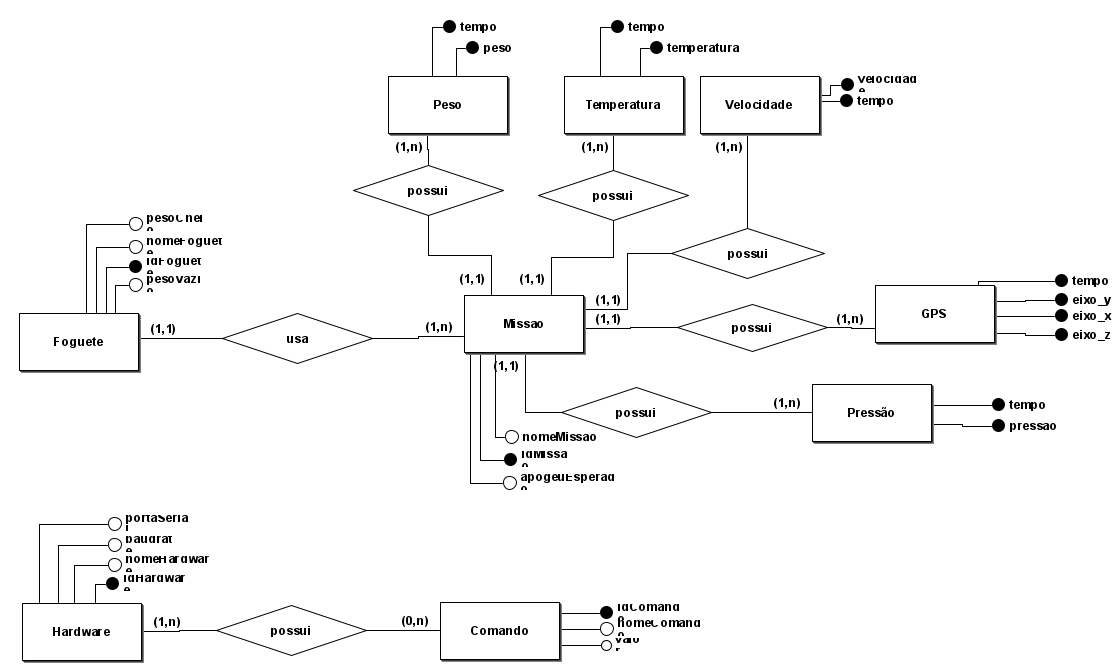
\includegraphics[keepaspectratio=true,scale=0.4]{figuras/conceitual_ground_station.png}
	\caption{Modelo Conceitual da modelagem.}
	\label{fig:conceitual}
\end{figure}


\begin{figure}[h!]
	\centering
	\label{server-side}
		\includegraphics[keepaspectratio=true,scale=0.4]{figuras/Lógico_ground_station.png}
	\caption{Modelo Lógico da modelagem}
	\label{fig:logico}
\end{figure}

Em seguida, foi gerado o modelo lógico da implementação para representar as tabelas junto com as chaves primarias e estrangeiras. A Figura \ref{fig:logico} apresenta essa implementação.

\subsection{Metas e restrições de arquitetura}
\label{metas_restricoes}

\subsubsection{Metas}
\begin{itemize}
    \item Auxiliar o usuário no lançamento e acompanhamento de voo de um foguete experimental.
    \item Armazenar dados dos lançamentos de forma sistemática.
    \item Ter uma interface intuitiva e de fácil utilização, para agilizar o processo de lançamento do foguete e análise dos dados pós voo.
    \item Possibilitar o controle do lançamento e acompanhamento do voo do foguete.
\end{itemize}

\subsubsection{Restrições}
\begin{itemize}
    \item O sistema não terá acesso a internet.
    \item Deve ser executado em microcomputador com recursos limitados.
    \item Realizar  \textit{streaming} de dados obtidos do foguete em tempo de execução.
    \item Disponibilizar dados armazenados em CSV para exportação via cartão SD.
    \item Utilizar ambiente conteinerizado (Docker) para virtualização do ambiente, a fim de poder simular o comportamento do software, já que não teremos a placa para fazer os testes.
    \item Deve ser utilizado um computador de arquitetura 64 bit ARM (Arm64) e um sistema operacional compatível.
\end{itemize}


%\subsubsection{Diagrama de pacotes}










